\chapter{Método Proposto}



% -.~.-.~.-.~.-.~.-.~.-.~.-.~.-.~.-.~.-.~.-.~.-
\section{Visão geral}

O método proposto divide-se nas seguintes etapas:

\missingfigure[figheight=100mm]{Diagrama do método}


% -.~.-.~.-.~.-.~.-.~.-.~.-.~.-.~.-.~.-.~.-.~.-
\section{Modelo do robô}

Nesta seção, são detalhados os procedimentos para representar o manipulador
robótico como um conjunto MBS e utilizá-lo para simular as trajetórias
referentes a uma determinada tarefa. O manipulador será descrito pelo conjunto
de Sistemas de Coordenadas (SC's) referente a cada uma de suas juntas, pelas
distâncias entre os SC's e posição dos centros de massa de cada elo, e pelos
parâmetros de massa e momento de inércia de cada elo. Os elos do robô e a
ferramenta acoplada no efetuador representam cada corpo do sistema MBS. A
modelagem do manipulador é simplificada utilizando as rotinas de CAS
desenvolvida especialmente para MBS, o Sophia, assim como a notação algébrica de
Lesser, apresentada na seção~\ref{sec::sophia-kane}.

\subsection{Descrição do braço robótico}

O manipulador escolhido para estudo é o mesmo que será utilizado no projeto EMMA
para revestimento de superfícies metálicas por HVOF. Trata-se de um robô
comercial modelo MH12, da série MOTOMAN, fabricado pela Yaskawa Motoman
(Figura~\ref{fig::mh12_foto}).

\begin{figure}[h]
    \centering
    \begin{subfigure}[b]{0.3\textwidth}
        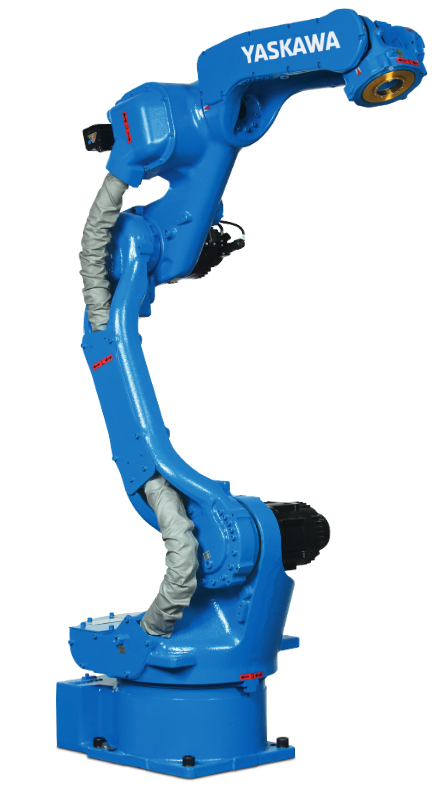
\includegraphics[width=\textwidth]{figs/mh12_foto}
        \caption{MOTOMAN MH12. \\Fonte: adaptada de}
        \label{fig::mh12_foto}
    \end{subfigure}
    \quad %add desired spacing between images, e. g. ~, \quad, \qquad, \hfill
    % etc.
      %(or a blank line to force the subfigure onto a new line)
    \begin{subfigure}[b]{0.5\textwidth}
        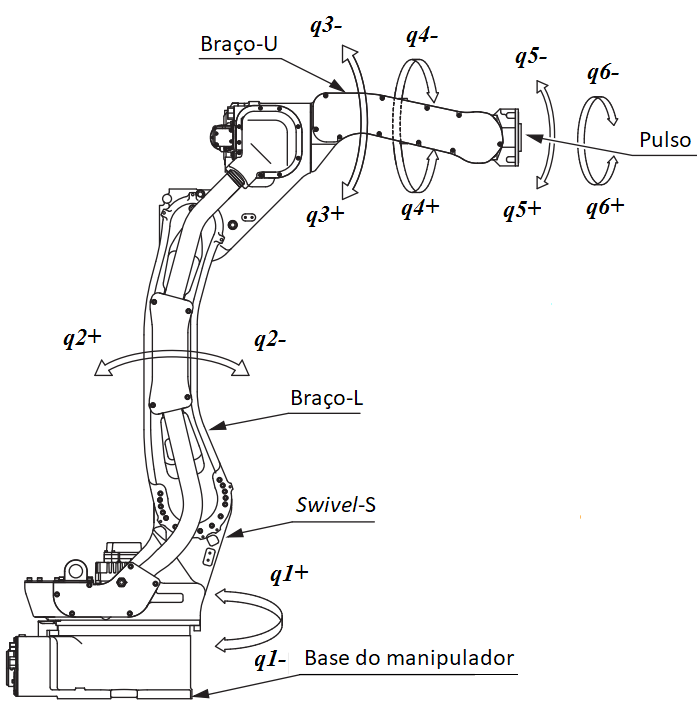
\includegraphics[width=\textwidth]{figs/mh12_diagram}
        \caption{Diagrama dos elos e juntas. \\Fonte: adaptada de}
        \label{fig::mh12_diagram}
    \end{subfigure}
    \caption{Manipulador robótico para modelo}\label{fig::resumo_mh12}
    \todo[inline]{Inncluir referências das figuras - MH12 specsheet}
\end{figure}

\begin{table}[h]
\centering
\caption{Sistemas de coordenadas, elos e coordenadas generalizadas}
\label{tab::resumo_mh12}
\begin{tabular}{@{}clc@{}}
\toprule
SC & Elo              & \multicolumn{1}{l}{Coord. gen. associada} \\ \midrule
Z  & Pedestal do robô & -                                         \\
S  & \textit{Swivel}  & q1                                        \\
L  & Braço inferior   & q2                                        \\
U  & Braço superior   & q3                                        \\
R  & Braço de rolagem & q4                                        \\
B  & Pulso            & q5                                        \\
T  & Efetuador        & q6                                        \\ \bottomrule
\end{tabular}
\end{table}

Este robô é um braço antropomórfico de 6 juntas rotacionais e portanto 6 graus
de liberdade (6 gdl), contendo o último elo um porta-ferramentas que suporta uma
carga útil de até 12 kg. A Figura~\ref{fig::mh12_diagram} apresenta os nomes dos
elos e coordenadas generalizadas associados a cada um dos sistemas de
coordenadas e são resumidos na Tabela~\ref{tab::resumo_mh12}.

O alcance horizontal deste manipulador chega a 1,440~m, e vertical a
2,511~m. Estão representados no diagrama do espaço de trabalho na
Figura~\ref{fig::workspace} em que a área sombreada é formada por todos os
pontos alcançáveis pelo manipulador, dentro dos limites de cada junta.

\begin{figure}[h]
	\centering 
 	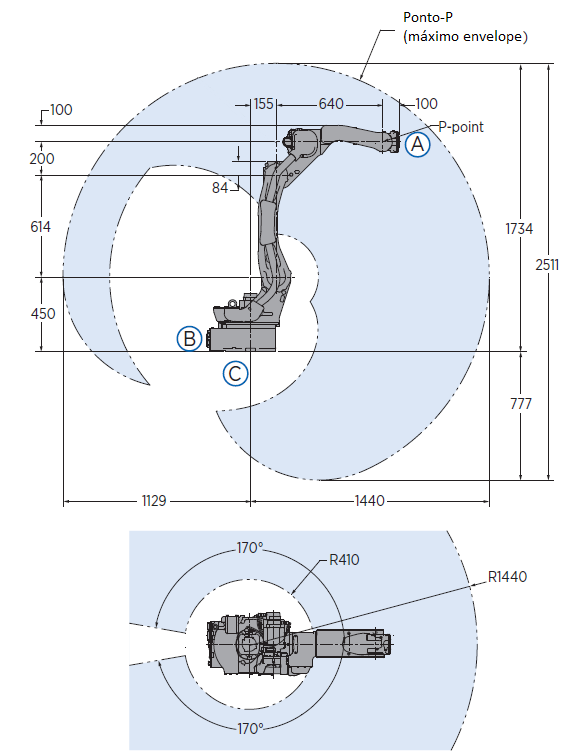
\includegraphics[width=0.7\textwidth]{figs/workspace}
 	\caption{Vistas lateral e superior do espaço de trabalho. \\Fonte: adaptada
 	de}
 		\todo[inline]{Inncluir referência da figura - MH12 specsheet}
 	\label{fig::workspace}
\end{figure}

Conforme discutido na seção~\ref{sec::manind}, este tipo de braço robótico
permite desacoplar o sistema em 2 problemas: posicionamento e orientação. Logo,
para simplificar o modelo e o cálculo da cinemática inversa, serão consideradas
as 3 primeiras juntas para posicionamento e 3 últimas (pulso esférico) para
orientação da ferramenta.

A última junta, no efetuador, tem a finalidade de orientar a ferramenta em torno
do seu eixo axial. Como o processo de revestimento por HVOF independe desta
orientação, esta junta não será incluída, mantendo este acoplamento rígido, o
que transforma os dois últimos elos em apenas um corpo.
Como resultado, tem-se um sistema de 5 gdl.


\subsection{Cinemática Direta}

Como foi discutido na seção~\ref{sec::cinematica}, o procedimento mais utilizado
para a modelagem cinemática de manipuladores robóticos é o método dos parâmetros
de Denavit-Hartenberg (parâmetros D-H). Apesar de sua popularidade e vasta
utilização na modelagem cinemética de manipuladores variados, este método possui
regras que acabam restringindo uma livre escolha dos sistemas de coordenadas e
as direções dos eixos de referência. Dependendo da geometria do robô, pode ser
uma tarefa trabalhosa definir os parâmetros e referenciais mais convenientes, e
que resultem num sistema final simplificado.

Um maior controle sobre a escolha dos referenciais e dos parâmetros da geometria
pode reduzir significativamente o custo computacional do modelo.
Neste sentido, o Sophia-Maple é uma ferramenta mais genérica, que permite, ao
usuário, total liberdade sobre a escolha dos referenciais, sem nenhum aumento de
complexidade. Uma escolha estratégica da posição e orientação dos sistemas de
coordenadas pode resultar em equações cinemáticas e transformações de
referenciais mais simplificadas. Neste trabalho serão utilizadads as rotinas do
Sophia para modelagem da cinemática direta do manipulador robótico.

\todo[inline]{Incluir parágrafo sobre cálculo diff e vetor tangente tau}

\subsubsection{Sistemas de Coordenadas e Transformações Homogêneas}

A primeira etapa para obter-se as equações cinemáticas será definir o sistema de
coordenadas fixo em cada elo do robô. A Figura~\ref{fig::scs} é um modelo CAD do
manipulador e apresenta a posição de cada SC, na configuração inicial.

\begin{figure}[h]
    \centering
    \begin{subfigure}[b]{0.20\textwidth}
        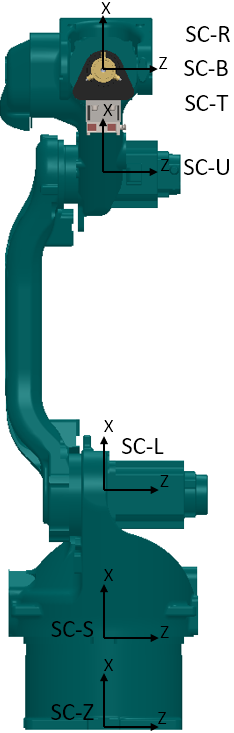
\includegraphics[width=\textwidth]{figs/sc_front}
        \caption{Vista frontal}
        \label{fig::sc_front}
    \end{subfigure}
    \quad %add desired spacing between images, e. g. ~, \quad, \qquad, \hfill
    % etc.
      %(or a blank line to force the subfigure onto a new line)
    \begin{subfigure}[b]{0.7\textwidth}
        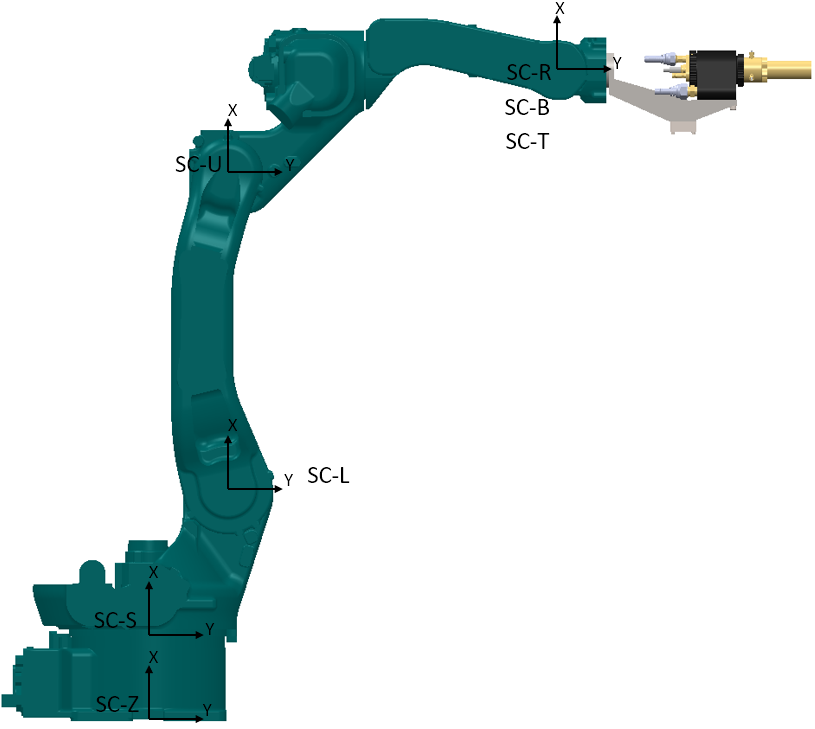
\includegraphics[width=\textwidth]{figs/sc_lat}
        \caption{Vista lateral}
        \label{fig::sc_lat}
    \end{subfigure}
    \caption{Sistemas de coordenadas do robô}\label{fig::scs}
\end{figure}

Na vista frontal (Figura~\ref{fig::sc_front}) nota-se que foi escolhida uma
configuração em que todos os SC's estivessem no mesmo plano XY. Outra observação
é que os SC's R, B e T estão fixados no mesmo ponto. que representa a
origem do ``pulso'' do braço robótico. Estas considerações reduzem a quantidade
de termos das equações cinemáticas. Além disso, serão muito importantes para o
cálculo da cinemática inversa, como será visto na seção~\ref{sec::ikin_mh12}.

Logo, pode-se escrever as relações entre estes referenciais em termos das
coordenadas generalizadas do sistema, para obter as transformações entre cada
SC. No Sophia-Maple isto é feito com o uso da função \textit{chainSimpRot}, da
seguinte forma:

\noindent {\tt > chainSimpRot( [Z,S,1,q1], [S,L,3,q2], [L,U,3,q3], [U,R,2,q4],
[R,B,3,q5], [B,T,2,q6] )}

Esta função cria as matrizes de rotação entre os referenciais do sistema,
informando a cada transformação, o eixo de rotação
(onde 1=X, 2=Y e 3=Z) e a coordenada generalizada associada
(q1,~\ldots~,q6). Foi utilizada a forma de coordenadas relativas entre cada SC.
Logo, como exemplo o termo {\tt [L,U,3,q3]} representa uma rotação de um ângulo
q3, do SC-U em relação ao SC-L, em torno do eixo Z.

Logo, como exemplo, a matriz Transformação Homogênea
entre o referencial inercial Z e o braço superior U seria:
%
$$ R_{Z}^{U} = R_{Z}^{S} R_{S}^{L} R_{L}^{U} $$
%
A função \textit{Rmx} do Sophia-Maple retorna a matriz de rotação entre quaisquer
sistema de coordenadas. No Sophia-Maple, escreve-se:

\noindent {\tt > Rmx(Z,U)}

E o resultado é:
%
$$ R_{Z}^{U} = \left[ \begin {array}{ccc} {\it c2}\,{\it c3}-{\it s2}\,{\it
s3}&-{ \it c2}\,{\it s3}-{\it s2}\,{\it c3}&0\\ \noalign{\medskip}{\it c1}\,{
\it c2}\,{\it s3}+{\it c1}\,{\it s2}\,{\it c3}&{\it c1}\,{\it c2}\,{
\it c3}-{\it c1}\,{\it s2}\,{\it s3}&-{\it s1}\\ \noalign{\medskip}{
\it s1}\,{\it c2}\,{\it s3}+{\it s1}\,{\it s2}\,{\it c3}&{\it s1}\,{
\it c2}\,{\it c3}-{\it s1}\,{\it s2}\,{\it s3}&{\it c1}\end {array}
 \right] $$
 %
 A matriz acima foi escrita em notação trigonométrica simplificada, em que c1,
 s1, ,c2, s2, \ldots, e assim por diante representam as funções senos e cossenos
 dos ângulos das coordenadas generalizadas q1, \ldots, q5. Para melhor
 visualização das matrizes e equações, esta notação será utilizada em todo o
 trabalho.
 
\subsubsection{Vetores posição e centros de massa}

A segunda etapa é definir os vetores posição dos centros de massa de cada corpo.
Para isso, define-se auxiliarmente os vetores posição entre cada SC, desde o
referencial inercial Z até o efetuador em T. Será utilizada a notação de Lesser,
por meio dos \textit{Evectors}, como descrito na seção~\ref{sec::sophia-kane}
para representar esses vetores.

Logo, de maneira geral, pode-se escrever a posição de qualquer ponto pela
seguinte relação:
%
\begin{align}
	^{Z}\mathbf{p}^{k} = ^{Z}\mathbf{p}^{k-1} + ^{k-1}\mathbf{p}^{k} \\
	^{Z}\mathbf{pcm}^{k} = ^{Z}\mathbf{pcm}^{k-1} + ^{k}\mathbf{pcm}
	\label{eq::pcm}
\end{align}
%
Onde $^{Z}\mathbf{p}^{k}$ é o vetor posição do referencial $k$ em relação ao
referencial inercial $Z$ e analogamente $^{Z}\mathbf{pcm}^{k}$ é o vetor
posição do centro de massa do corpo $k$, tal que $k$ varia em \{S,L,U,B,T\}.
No Sophia-Maple escreve-se:

\noindent {\tt > pZ:= Evector(0,0,0,Z)} \\
\noindent {\tt > for k from corpo[1] to corpo[6] do \\
\indent p||k:= p||{k-1} \&++ Evector(p||{k-1}||{k}||x, p||{k-1}||{k}||y,
\indent p||{k-1}||{k}||z, k-1) \\
end do}

E para os centros de massa:

\noindent {\tt > for k from corpo[1] to corpo[6] do \\
\indent pcm||k:= p||{k} \&++ Evector(pcm||{k}||x, pcm||{k}||y, pcm||{k}||z, k)
\\ end do}

\subsubsection{Velocidades}

As velocidades dos centros de massa de cada corpo são calculadas como a derivada
do vetor posição com respeito ao referencial inercial. Logo, a derivada da
equação~\ref{eq::pcm} em Z:
%
\begin{equation}
	\mathbf{V}^{k} = \frac{^{Z}\mathrm{d} }{\mathrm{d} t}
	\mathbf{pcm}^{k} \label{eq::veloc}
\end{equation}
%
O Sophia-Maple possui um poderoso conjunto de rotinas para diferenciação dos
\textit{Evectors} com relação ao referencial inercial, por meio da função
\textit{cdft}, que reconhece automaticamente o referencial em que cada vetor
está descrito e realiza o cálculo diferencial vetorial. Logo, pode-se escrever o
seguinte comando para definir as velocidades de acordo com a
equação~\ref{eq::veloc}:

\noindent {\tt > for k from corpo[1] to corpo[6] do \\
\indent v||k:= cdft(pcm||{k}, Z) \\
end do}

As velocidades angulares serão a taxa de variação angular entre os referenciais




\subsection{Dinâmica}

\lipsum[1-1]

\subsection{Cinemática Inversa}\label{sec::ikin_mh12}

\subsection{Tarefa e trajetória}

\subsection{Modelo teórico MBS -- Robô}


% -.~.-.~.-.~.-.~.-.~.-.~.-.~.-.~.-.~.-.~.-.~.-
\section{Modelo da base}

\subsection{Geometria e CAD}

\subsection{Matriz de Rigidez}

\subsection{Matriz de Amortecimento}

\subsection{Análise Elementos Finitos}

\subsection{Modelo teórico MBS -- Base}


% -.~.-.~.-.~.-.~.-.~.-.~.-.~.-.~.-.~.-.~.-.~.-
\section{Ensaio Experimental}

\subsection{Bancada experimental}

\subsection{Programas de aquisição dos dados experimentais}

\subsection{Tratamento dos dados}

\subsection{Cálculo dos parâmetros modais da estrutura}


% -.~.-.~.-.~.-.~.-.~.-.~.-.~.-.~.-.~.-.~.-.~.-
\section{Modelo acoplado robô e base}

\subsection{Base rígida}

\subsection{Base flexível}


% -.~.-.~.-.~.-.~.-.~.-.~.-.~.-.~.-.~.-.~.-.~.-
\section{Estudos de casos para avaliação do método}

\subsection{Trajetórias do efetuador}

\subsection{Base rígida}

\subsection{Base de testes}

\subsection{Base modular PRP}

\subsection{Base com pouca rigidez}
